\section{Architettura del servizio}
\label{sec:chapter_baking_service_architettura_servizio}

\begin{figure}[htb]
 \centering
 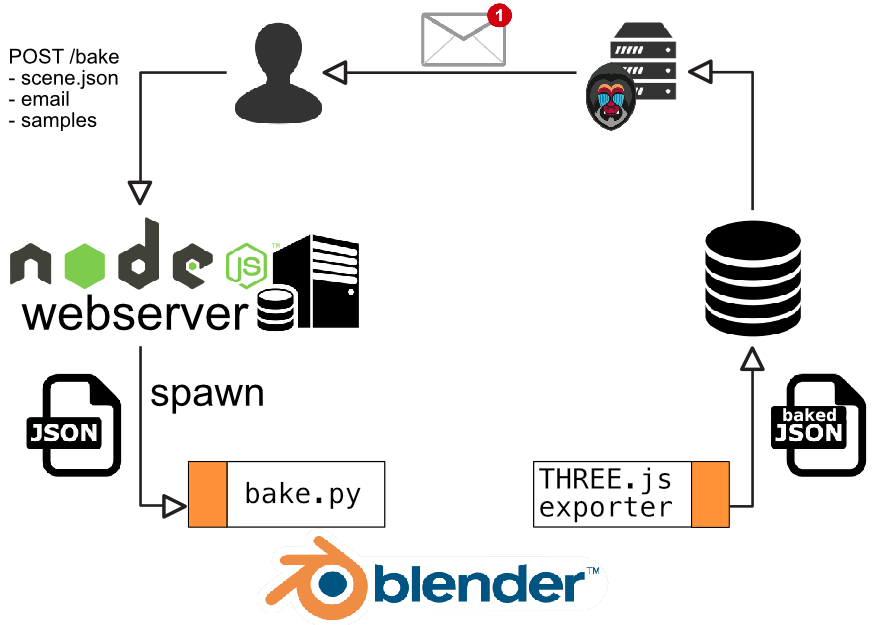
\includegraphics[width=1\linewidth]{images/chapter_baking_service/architettura.png}\hfill
 \caption[Architettura servizio di baking]{Descrizione generale dell'architettura del servizio, a fronte della sottomissione di una richiesta di bake da parte dell'utente.}
 \label{fig:architettura}
\end{figure}

Nella descrizione generale del servizio nel paragrafo \ref{sec:chapter_architettura_sistema_il_servizio_baking} si è accennato al fatto che le richieste sono elaborate dal server in modo differente a seconda del loro tipo, e che le elaborazioni più complesse possono essere decomposte in una successione di passi di elaborazione più piccoli. Ogni passo di elaborazione può essere implementato in una funzione separata, e ognuna di queste funzioni è detta Middleware. Ogni middleware è un componente autocontenuto che racchiude le responsabilità funzionali di implementare un passo di elaborazione.
\\
Questa caratteristica permette l’aggiunta o la rimozione di middleware dalla pipeline in modo agevole. Il flusso di dati in ingresso verrà elaborato attraverso i passi successivi della pipeline. 
\\
Il servizio prevede dunque un web server che ascolta le richieste dei client da remoto; questo web server è identificabile mediante indirizzo IP e numero di porta dalla quale è in ascolto; a fronte di una richiesta da parte del client manda in esecuzione una pipeline di middleware che la elabora, producendo una risposta. La pipeline di Middleware viene quindi invocata ogni volta che una richiesta HTTP viene catturata dal server. 
\\
Le richieste HTTP sottomesse dal client possono essere diverse, e quindi il server dovrà essere in grado di riconoscere che tipo di richiestà è, e quali sono le operazioni necessarie per soddisfarla. 
\\
Per ogni tipologia di richiesta ci sarà dunque una diversa pipeline di Middleware, ma non è detto che ci sia sempre bisogno di elaborare un flusso di dati mediante più passi di elaborazione; per operazioni semplici è infatti possibile definire un solo Middleware. 
Le diverse tipologie di richieste HTTP che il client può sottomettere sono mostrate in tabella:
\begin{table}[]
\centering
\caption[Richieste utente e middleware]{Tipi di richiesta utente e middleware}
\begin{tabular}{|l|l|l|l|l|}
\hline
\begin{tabular}[c]{@{}l@{}}Funzionalità\\ Editor\end{tabular} & \begin{tabular}[c]{@{}l@{}}Metodo \\ richiesta\end{tabular} & Contenuto & URL & Middleware \\ \hline
Bake & POST & \begin{tabular}[c]{@{}l@{}}scene.json, \\ email, \\ nome scena, \\ sampling\end{tabular} & /bake & \begin{tabular}[c]{@{}l@{}}validate\_parameters, \\ assign\_id, \\ create\_directory, \\ save\_input, \\ enqueue,  answer,\\ run\end{tabular} \\ \hline
Jobs & GET &  & /jobs & get\_jobs \\ \hline
Status & GET & \begin{tabular}[c]{@{}l@{}}id processo\\ bake\end{tabular} & /jobs:id & status \\ \hline
Delete & DELETE & \begin{tabular}[c]{@{}l@{}}id processo\\ bake\end{tabular} & /jobs:id & delete\_bake \\ \hline
\end{tabular}
\label{table:middleware_table}
\end{table}
Per diversificare le azioni in base alle richieste HTTP, il server è controllato da una tabella di routing, che associa a seconda del metodo e URL della richiesta, un certo numero di middleware, che sia una pipeline o uno singolo.
\\
All’arrivo di una richiesta HTTP il server confronta metodo e URL della richiesta con quelli presenti nella tabella di routing; se c’è una corrispondenza, allora il server invoca la pipeline di Middleware corrispondente. 
\\
Il Baking Service è realizzato con la consapevolezza che l’attività di modifica, aggiunta o rimozione di middleware può essere piuttosto frequente, pertanto si è cercato di individuare un framework che semplificasse questo tipo di operazioni. La soluzione è stata quella di realizzare un server HTTP basato su NodeJS. 
L’ambiente NodeJS, mostrato nel paragrafo \ref{sec:chapter_tecnologie_abilitanti_nodejs}, consente la realizzazione di applicazioni lato server in poche righe di codice, grazie a framework come \texttt{ExpressJS} \cite{node5} . Questo framework è lo standard de facto per la realizzazione di applicazioni server-side in ambiente Node, ed offre tutta una serie di strumenti per la realizzazione della routing table, e per la realizzazione dei middleware. 
\begin{figure}[htb]
 \centering
 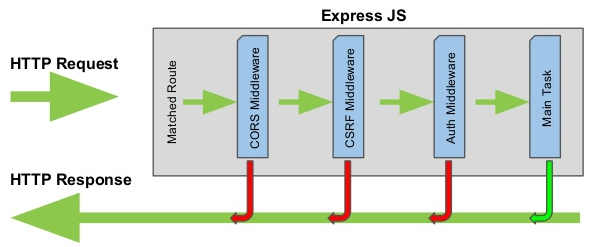
\includegraphics[width=1\linewidth]{images/chapter_baking_service/ba_se_ex_js.png}\hfill
 \caption[ExpressJS]{In foto un dettaglio sulla gestione delle richieste utilizzando un framework ExpressJS}
 \label{fig:ba_se_ex_js}
\end{figure}
Seguendo l’ordine della tabella, verranno ora analizzati i punti focali relativi alla realizzazione di ogni middleware, iniziando appunto dalla pipeline per processamento del bake. 
\\
Il primo passo della pipeline prevede che tutte le informazioni presenti nella POST vengano validate.
\\
Una volta validati i parametri vengono resi persistenti in una struttura dati contenente tutte le informazioni relative al processo di bake. Questo è necessario in quanto non solo ogni fase della pipeline di processamento ha bisogno di queste informazioni, ma come verrà mostrato più avanti in questo paragrafo, anche gli altri middleware mostrati in tabella ne faranno uso. 
\\
Viene dunque creata ed inizializzata una struttura \texttt{bake\_data} contenente le seguenti informazioni:
\begin{itemize}
\item Email utente, nome scena, e sampling (estratti dalla richiesta).
\item Istante di accettazione della richiesta (viene fatto coincidere con il momento in cui viene creata la struttura dati. Questo dato è utile per conoscere ad esempio il tempo che intercorre tra accettazione della richiesta, e l’inizio del processamento del bake).
\end{itemize}
Il passo di elaborazione successivo si occupa di assegnare un id univoco al processo di bake, memorizzandolo nel rispettivo bake\_data. L’id univoco è fondamentale per creare una corrispondenza tra client e processo di bake richiesto dal client, utile specialmente per le funzionalità Jobs, Status, e Delete.
\\
Successivamente bisogna rendere persistente su disco la scena fornita dall’utente; siccome il formato delle richieste di bake è sempre lo stesso, bisogna diversificare gli input in base al processo.
\\
Per prima cosa viene quindi creata nel file system una directory avente per nome l’id del processo. Il path della directory appena creata verrà memorizzato nei bake\_data del processo.
L’operazione successiva prevede la scrittura del file di input, ovvero la scena, all’interno di questa directory.
\\ 
A questo punto la fase di preprocessamento è conclusa, e può così iniziare la fase principale, ovvero il bake. Per i motivi gia discussi nei capitoli precedenti questa è ovviamente la fase più pesante e che richiede il maggior tempo per essere processata; fungerà quindi da collo di bottiglia per tutta la pipeline. Durante il processamento di un bake è possibile che le richieste per altri bake continuino ad arrivare, pertanto è necessario disciplinare gli arrivi in una struttura dati a coda. 
\\
Il server continuerà quindi ad accettare richieste, e per ognuna eseguirà tutti i passi di preprocessamento sopra mostrati; al termine di questi il processo di bake, rappresentato dai rispettivi bake\_data, verrà inserito all’interno di una coda. La disciplina è semplicemente quella di processare il primo bake in coda una volta concluso quello in esecuzione; per la realizzazione di questa disciplina è stato necessario trovare un modo per notificare al gestore della coda che può servire il prossimo bake. Per fare ciò il modo più corretto è quello di far notificare il termine del processo di bake direttamente al processo stesso, mediante invocazione di una callback al concludersi del processo. La callback viene ascoltata dal gestore, che quindi si impegnerà a controllare se ci sono delle richieste in coda, e in caso di elaborare la prima di queste. 
\\
A seguito dell’estrazione di una richiesta dalla coda può avere inizio il processo più importante, ovvero la fase di bake. 
\\
Questa fase prevede che alla fine, nella stessa directory generata nei passi precendenti, sia presente anche un file di output, contenente la scena con le lightmap. 
\\
Per comprendere la fase è necessario discutere un particolare circa il software di grafica 3D utilizzato. Uno dei motivi per cui è stato scelto Blender, è la possibilità che ha di essere invocato direttamente da console di comando sottomettendo una stringa contenente, oltre alla chiamata al processo Blender, un path del file contenente la lista di comandi che deve svolgere. 
\\
Questo metodo automatizza completamente l’esperienza d’uso con Blender, in quanto il processo seguirà la lista dei comandi senza bisogno di interazione da parte dell’utente.
\\ 
Ciò di cui si occupa la fase di bake è automatizzare anche la sottomissione di questa stringa sulla console dei comandi. La sottomissione è fatta mediante lo spawn di un processo figlio a quello che si occupa della fase di bake; a questo processo figlio viene associato il path del processo in cui si deve trasformare, ossia Blender, e una stringa contenente:
\begin{itemize}
\item Lo script che Blender deve eseguire (\ref{sec:chapter_baking_service_pipeline_baking_caricam_scena}).
\item Il path locale, estratto dai bake\_data, dove è memorizzata la scena.
\item Il path locale dove memorizzare l’output.
\item Il sampling, anch’esso estratto dai bake\_data.
\end{itemize}
A questo punto il processo sarà completamente autonomo ed inizierà la procedura di baking sulla scena. Durante l’esecuzione del bake bisogna poter ascoltare il processo, in modo ad esempio da poter individuare il motivo di un’eventuale fallimento dello stesso. Il modo migliore per farlo è quello di realizzare dei log di sistema per ogni processo di bake che verrà lanciato.
\\ 
Per questo motivo la prima attività in cui si impegna la fase di bake è la creazione di due file di log all’interno della stessa directory usata per l’input e per l’output del processo di bake. Di questi due log uno conterrà eventuali errori, e quindi sarà la destinazione per i messaggi di errore del processo,lo \texttt{stderr}; l’altro log sarà invece la destinazione per i messaggi di sistema del processo, quindi lo \texttt{stdout}. 
Questo secondo log in particolare è l’unico strumento in possesso per interrogare il processo, e chiedere ad esempio il suo stato di completamento. 
\\
Durante la scrittura dello stdout nel log, è possibile infatti deviare il flusso attraverso un filtro: questo filtro attua un processo di riconoscimento di template di stringhe all’interno del flusso.
\\ 
Il processo di Blender che genera gli stdout e stderr durante l’esecuzione, viene istruito affinchè per ogni lightmap processata produca una stringa contenente il numero di lightmap che fino a quel momento ha processato sul totale di lightmap che deve produrre. 
Questa stringa ha un template noto al filtro, che quindi la riconosce, estrae l’informazione di completamento, e la memorizza nei bake\_data del processo. In questo modo l’utente può venire a conoscenza dello stato di completamento del bake. 
\\
Al termine del processo di bake viene calcolata la durata complessiva del processo, e memorizzata nei bake\_data insieme al codice di uscita del processo, che può essere 0 (esito positivo), o 1 (errore nel processo).
\\ 
L'ultimo passo prevede la creazione e l'invio della mail all'utente. Utilizzando le API offerte da un servizio di mailing viene creato un tipo diverso di mail a seconda dell’esito del bake; la mail viene poi spedita all’indirizzo memorizzato nei bake\_data. 
\\
Se il processo di bake è terminato correttamente, la mail conterrà l’URL per scaricare l'output del processo, ossia la scena con le lightmap. Se l’esito è negativo la mail conterrà un messaggio di errore specifico in base al fallimento riscontrato.
\\
Per quanto riguarda la gestione delle Email, è stato necessario individuare uno strumento che consentisse la creazione e l’invio di email transazionali da applicazione web in modo del tutto automatico. 
\\
Le e-mail transazionali sono e-mail che vengono spedite all’utente in base ad una qualche azione. L’azione può essere innescata direttamente dall’utente, oppure può avere come target l’utente stesso. La conferma di un indirizzo email, la richiesta di reimpostare una password o una conferma di pagamento sono solo alcune delle azioni che possono scatenare l’invio di una email transazionale. 
\\
Il grande vantaggio di questo tipo di email è che sono configurate in modo che l’azione scatenante causi l’invio dell’ email in real-time, entro pochi secondi dopo l’azione. Nel contesto del presente lavoro di tesi l’azione scatenante per l’invio di una mail è l’esecuzione del processo di bake. 
\\
Per la creazione e l’invio di email transazionali sono state utilizzate le API offerte dal servizio Mandrill, un’infrastruttura per l’invio di e-mail semplice da utilizzare e ben documentata.
\\
Terminata la descrizione del Middleware che si prende carico dell'elaborazione delle richieste di bake, seguendo la tabella \ref{table:middleware_table} verrà ora fornita una descrizione dei Middleware per l'elaborazione degli altri tipi di richieste che l'utente può sottomettere al servizio.
\\ 
In qualsiasi momento durante l’utilizzo dell’editor, l’utente ha la possibilità di interrogare il servizio di Baking per sapere quante richieste di bake sta elaborando. 
\\
Questa richiesta viene passata dal server HTTP al middleware che si occuperà di copiare in una lista tutti i bake\_data delle richieste di bake in coda in attesa di essere processate, insieme al bake\_data del processo attualmente in esecuzione. 
Questa lista verrà inviata in risposta al client, che si occuperà di mostrare sull’editor i nomi dei processi.
\\
L’utilità di restituire al client la lista con tutti i bake\_data sta nel fatto che una futura esigenza di utilizzare lato client un’informazione diversa presente nei bake\_data non richiederà alcuna modifca lato server. 
\\
Per ogni processo che l’editor mostra all’utente, vengono offerte due funzionalità: chiedere lo stato di esecuzione della richiesta, o annullarla. Per funzionalità di questo tipo diventa essenziale mantenere nell’editor gli id dei processi mostrati all’utente.
Questo perchè al momento della sottomissione di una delle due richieste al server, questo deve essere in grado di riconoscere il processo per il quale è stato chiesto lo status, o l’eliminazione. 
\\
Per quanto riguarda l’elaborazione della richiesta di status da parte del server, la prima cosa che il middleware fa è estrarre l’informazione chiave, ovverò l’id del processo. Da questo momento in poi il middleware si impegna nel determinare lo stato della richiesta individuando a che punto si trova nel suo ciclo di vita. 
\\
Il ciclo di vita di una richiesta di bake prevede una fase precedente all’inserimento in coda, una fase durante l’attesa in coda, e un’ultima fase dopo l’estrazione dalla coda. In ognuna di queste fasi i bake\_data della richiesta possono trovarsi in luoghi differenti. 
\\
Per prima cosa si controlla se i bake\_data con quell’id si trovano in coda di attesa. In tal caso viene preparato il messaggio di risposta per l’utente contenente la notifica del fatto, insieme ad una stima del numero di processi che precedono nella coda quello richiesto. 
\\
Si parla di stima in quanto dalla sottomissione della richiesta dell’utente, alla ricezione della risposta, la situazione nella coda potrebbe essere cambiata. Tuttavia trattandosi il bake di un processo tipicamente lento, la stima è una buona approssimazione della realtà. 
\\
Se questo primo controllo fallisce, è possibile che la richiesta non sia in attesa perchè gia in esecuzione. A questo punto vengono controllati i bake\_data del processo in esecuzione, i quali vengono marcati come tali nel momento esatto in cui l’istanza di Blender inizia il bake.
\\ 
Se il bake\_data contiene l’id che si sta cercando, allora non solo verrà notificato all’utente lo stato di esecuzione in corso, ma verrà notificata anche la percentuale di completamento del processo, estratta dai bake\_data e calcolata mediante il parsing dello stdout mostrato in precedenza.
\\ 
Se ancora non c’è una corrispondenza con l’id del processo in esecuzione, l’unica possibilità è che il processo sia già terminato da tempo. A questo scopo il sistema mantiene uno storico dei processi di bake terminati, che quindi può essere consultato in ricerca dei bake\_data. Se la ricerca ha esito positivo l’utente verrà notificato a riguardo, esortandolo a controllare le sue mail. 
\\
Per quanto riguarda l’elaborazione della richiesta di eliminazione di un bake, anche in questo caso il middleware si impegna dapprima nell’estrazione dell’id dalla richiesta. 
\\
A questo punto viene effettuata una ricerca su due fronti: o il processo è in attesa in coda, e quindi l’annullamento del processo corrisponderà semplicemente nel rimuovere dalla coda i rispettivi bake\_data, facendo avanzare tutte le richieste antecedenti, o il processo è già in esecuzione. In questo secondo caso bisognerà arrestare il processo di Blender, inviandogli un segnale di terminazione. 
Una volta fermato il processo, il gestore della coda provvederà a soddisfare la richiesta successiva.    